Questo capitolo descrive l'implementazione tecnica della soluzione architetturale progettata nel Capitolo \ref{chap:analisi}. La trattazione segue un approccio bottom-up, partendo dalla base infrastrutturale fino ad arrivare agli strumenti di automazione per gli sviluppatori.  La prima fase dell'implementazione riguarda la traduzione della topologia cloud in codice Terraform, necessaria per istanziare gli ambienti di base. Successivamente, il capitolo dettaglia la scrittura del codice applicativo, separando i processi asincroni del livello dati dall'implementazione delle API sincrone di backend. Una volta definiti i componenti cloud e applicativi, la trattazione si sposta sulle metodologie adottate per garantire la testabilità del codice sulla workstation dello sviluppatore tramite emulazione locale. Il consolidamento di questi processi culmina nell'implementazione delle pipeline di Continuous Integration e Continuous Deployment, che eliminano l'intervento manuale nei rilasci. Infine, illustra lo sviluppo di Service-Forge, il framework interno creato per automatizzare la generazione di nuovi microservizi interfacciando l'infrastruttura prodotta con agenti basati su Large Language Models.

\section{Provisioning dell'Infrastruttura tramite Terraform}

L'adozione di un approccio Infrastructure as Code (IaC) garantisce la riproducibilità, la tracciabilità e la coerenza degli ambienti cloud. Il repository oggetto di questa sezione traduce la topologia cloud, descritta nei capitoli precedenti, in codice HCL (HashiCorp Configuration Language), il linguaggio dichiarativo utilizzato da Terraform per definire risorse infrastrutturali. Ogni componente trova una corrispondenza diretta in moduli Terraform versionati e organizzati secondo una struttura gerarchica.

Come discusso nel Capitolo \ref{chap:analisi}, la scelta di Terraform come strumento di provisioning deriva da tre fattori tecnici: la natura dichiarativa del linguaggio, che delega al motore il calcolo del piano di esecuzione; il supporto multi-provider, essenziale per gestire risorse AWS, Google Cloud Platform e MongoDB Atlas in un singolo repository; e l'ecosistema di moduli riutilizzabili.

La gestione dello stato per ambienti multipli richiede l'utilizzo di Terragrunt come orchestratore. Terragrunt opera come wrapper per Terraform, aggiungendo funzionalità di gestione dello stato remoto, generazione automatica di file di configurazione e risoluzione delle dipendenze tra moduli \cite{Terragrunt}. Questa combinazione applica il principio Don't Repeat Yourself alla definizione dell'infrastruttura.

La struttura logica di questa sezione segue il flusso di astrazione dell'infrastruttura: la scomposizione iniziale del repository illustra la separazione tra configurazione e implementazione; le sezioni successive dettagliano l'orchestrazione dello stato, la segregazione degli ambienti (multi-account) e, infine, la logica interna dei moduli riutilizzabili sviluppati per la piattaforma.

\subsection{Struttura del Repository}

Il repository implementa una separazione netta tra tre livelli logici, come illustrato in Figura \ref{fig:architettura_repo_devops}: le configurazioni Terragrunt specifiche per ambiente (directory \texttt{infra/}), le definizioni delle risorse Terraform raggruppate per dominio funzionale (directory \texttt{resources/}) e i moduli riutilizzabili (directory \texttt{utils/modules/}).

\begin{lstlisting}[basicstyle=\ttfamily\small, breaklines=true, columns=fullflexible]
devops-farm-tf/
|-- infra/                          # Configurazioni Terragrunt
|   |-- root.hcl                    # Configurazione globale
|   |-- _env/                       # Template di modulo (env-agnostic)
|   |   |-- 000-commons.hcl
|   |   |-- 010-networkings.hcl
|   |   |-- 020-messaging.hcl
|   |   |-- 050-integrations.hcl
|   |   |-- 060-mongodb.hcl
|   |   |-- 070-microservices.hcl
|   |   +-- 090-dwh.hcl
|   |-- dev/                        # Ambiente di sviluppo
|   |   |-- env.hcl
|   |   |-- 000-commons/
|   |   |-- 010-networkings/
|   |   |-- 020-messaging/
|   |   |-- 070-microservices/
|   |   +-- ...
|   |-- prod/                       # Ambiente di produzione
|   +-- shared/                     # Account condiviso
|       |-- main/                   # Organizzazione AWS
|       +-- shared/                 # Risorse condivise (ECR, domini)
|
|-- resources/                      # Definizioni Terraform per dominio
|   |-- 000-commons/                # OIDC GitHub, API GCP, IAP
|   |-- 010-networkings/            # VPC, subnet, NAT Gateway
|   |-- 020-messaging/              # Topic SNS
|   |-- 050-integrations/           # Service account GCP
|   |-- 060-mongodb/                # Cluster MongoDB Atlas
|   |-- 070-microservices/          # Cognito, Lambda, ECS, S3, DynamoDB
|   |-- 090-dwh/                    # Athena, Glue, Data Warehouse
|   |-- main/                       # AWS Organizations, SSO, IAM
|   +-- shared/                     # ECR, domini Route53
|
+-- utils/modules/                  # Moduli Terraform riutilizzabili
    |-- api-gateway-lambda/         # API Gateway HTTP + Lambda + Cognito
    |-- datasource-etl/             # Pipeline ETL: Extr + Tran + Glue + Athena
    |-- scheduled-lambda/           # EventBridge + Lambda schedulata
    +-- sns-consumer-lambda/        # SNS -> Lambda consumer
\end{lstlisting}

La numerazione progressiva delle directory sotto \texttt{resources/} (es. 000, 010, 020) riflette rigorosamente l'ordine di applicazione delle risorse e le dipendenze logiche: le risorse di rete (010) precedono il deployment dei microservizi (070).

\begin{figure}[htbp]
    \centering
    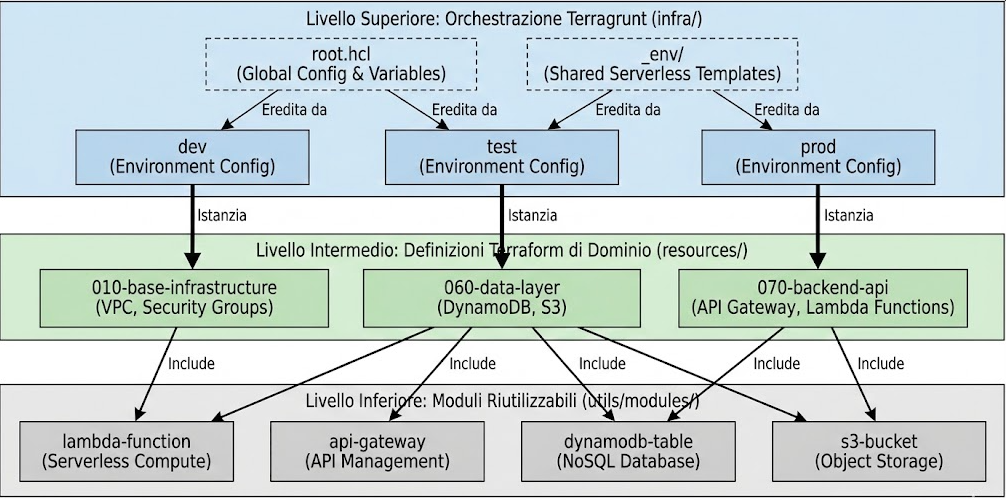
\includegraphics[width=1\textwidth]{images/architettura_repo_devops.png}
    \caption{Architettura logica del repository di Infrastructure as Code. Il diagramma illustra la gerarchia di orchestrazione tra le configurazioni di ambiente gestite tramite Terragrunt (livello superiore), le definizioni dei domini funzionali (livello intermedio) e i moduli Terraform di base riutilizzabili (livello inferiore) [Elaborazione dell'autore].}
    \label{fig:architettura_repo_devops}
\end{figure}

\subsection{Orchestrazione con Terragrunt}

Terragrunt introduce un livello di astrazione che risolve la configurazione del backend remoto, la generazione dei file provider e la gestione delle dipendenze tra moduli.

\subsubsection{Gestione dello Stato Remoto e Provider}

Lo stato di Terraform contiene la mappatura tra le risorse dichiarate nel codice e quelle allocate nel cloud. Per garantire persistenza, cifratura server-side e mutua esclusione durante le operazioni concorrenti, il repository utilizza un backend Amazon S3 con meccanismo di lock affidato ad Amazon DynamoDB.

Terragrunt genera automaticamente il file \texttt{provider.tf} per ogni modulo. La piattaforma richiede tre provider AWS distinti e un provider Google Cloud per gestire risorse eterogenee.

\subsubsection{Gerarchia di Inclusione e Dipendenze}

Ogni modulo in un ambiente specifico è rappresentato da un file \texttt{terragrunt.hcl} che combina la configurazione globale con il template del modulo e le dipendenze specifiche. Questa composizione a tre livelli (root, template, ambiente) centralizza la logica. Ad esempio, il blocco \texttt{dependency} consente di estrapolare gli output di un modulo già applicato (es. l'infrastruttura di messaggistica) e passarli come input al modulo corrente (es. i microservizi).

\subsection{Architettura Multi-Account}

La piattaforma opera su un'organizzazione AWS composta da ambienti segregati (dev, prod, shared), la cui topologia è schematizzata in Figura \ref{fig:aws_multi_account_topology}. L'utilizzo del servizio AWS Organizations permette di istanziare account separati, assegnando indirizzi email univoci e ruoli amministrativi per l'assunzione di identità cross-account.

L'accesso degli operatori è regolato tramite IAM Identity Center. Il modulo definisce gruppi e permission set specifici; ad esempio, il gruppo assegnato all'analisi dati riceve esclusivamente i permessi di lettura per interrogare il data warehouse tramite Amazon Athena, senza facoltà di modifica sulle risorse.

\subsection{Moduli Riutilizzabili}

La directory \texttt{utils/modules/} contiene i moduli Terraform che incapsulano i pattern architetturali ricorrenti.

\subsubsection{Modulo \texttt{api-gateway-lambda}}

Questo modulo rappresenta il pattern standard per il deployment dei microservizi serverless. Crea un endpoint HTTP (API Gateway v2), una funzione Lambda, un authorizer JWT \cite{JWT} opzionale basato su Amazon Cognito e i relativi gruppi di log in CloudWatch.

Un aspetto ingegneristico rilevante risiede nella separazione tra il ciclo di vita dell'infrastruttura e quello del codice applicativo. Nel blocco di definizione della funzione Lambda, l'attributo \texttt{image\_uri} viene escluso dal monitoraggio dello stato di Terraform:

\begin{lstlisting}[language=HCL]
resource "aws_lambda_function" "lambda" {
  function_name = "${var.name}-${var.env}"
  role          = aws_iam_role.lambda_assume_role.arn
  package_type  = "Image"
  image_uri     = var.app_image

  lifecycle {
    ignore_changes = [image_uri]
  }

  timeout       = var.lambda_timeout
  memory_size   = var.lambda_memory_size
  architectures = ["arm64"]

  environment {
    variables = merge(
      var.environments,
      {
        CLOUD_ENV = var.env
        STAGE     = "/api"
    })
  }
}
\end{lstlisting}

Questa direttiva impedisce a Terraform di ripristinare una versione precedente dell'immagine Docker qualora l'applicazione sia stata aggiornata in modo asincrono dalle pipeline di Continuous Deployment. La policy IAM della funzione viene costruita dinamicamente componendo i permessi di base (scrittura dei log) con istruzioni opzionali passate dal modulo chiamante, consentendo un'applicazione granulare del principio del minimo privilegio.

\subsubsection{Modulo \texttt{datasource-etl}}

Questo modulo definisce la pipeline ETL (Extract, Transform, Load) per l'ingestione dei dati. L'architettura di questo componente, dettagliata in Figura \ref{fig:pipeline-etl}, prevede una netta separazione fisica e logica dei dati: un prefisso S3 \texttt{raw/} per i dati grezzi e un prefisso \texttt{clean/} per i dati trasformati in formato Apache Parquet.

L'orchestrazione si divide in due fasi computazionali. La fase di estrazione (Extractor) utilizza una funzione Lambda invocata temporalmente tramite regole Amazon EventBridge. Per evitare la duplicazione dei dati grezzi in caso di errori temporanei della sorgente, i retry automatici dell'invocazione asincrona sono disabilitati (\texttt{maximum\_retry\_attempts = 0}).

La fase di trasformazione è puramente event-driven: viene attivata dalle notifiche S3 alla creazione di un nuovo oggetto nel prefisso \texttt{raw/}. Le policy IAM dei due componenti riflettono il flusso dei dati: l'Extractor ha permessi di sola scrittura su \texttt{raw/}, mentre il Transformer legge da \texttt{raw/} e scrive esclusivamente su \texttt{clean/}.

I dati elaborati vengono resi interrogabili tramite l'integrazione con AWS Glue Catalog e Amazon Athena. Il modulo implementa la funzionalità di Partition Projection per ottimizzare le query; le partizioni temporali (anno, mese, giorno) vengono calcolate matematicamente dal motore di Athena in base a range predefiniti, eliminando la necessità di eseguire operazioni di scansione sincrona (crawler) sui bucket S3.

\subsection{Risorse Condivise e Continuous Integration}

L'account condiviso ospita i repository Elastic Container Registry (ECR). L'accesso da parte dei sistemi di Continuous Integration (GitHub Actions) avviene senza lo scambio di credenziali, sfruttando il protocollo OIDC (OpenID Connect). Il provider di identità assume un ruolo IAM temporaneo che garantisce unicamente i permessi di push sui repository di destinazione.

\subsection{Strategia di Tagging}

Ogni risorsa gestita tramite IaC riceve un set di tag obbligatori (\texttt{terraform}, \texttt{environment}, \texttt{project}, \texttt{subproject}). Oltre all'identificazione visiva, questi metadati sono integrati con AWS Cost Explorer come Cost Allocation Tags, permettendo l'analisi e la ripartizione dei costi infrastrutturali per specifico dominio funzionale o ambiente.

\section{Sviluppo del Flusso ETL Event-Driven}
\label{sec:sviluppo-flusso-etl}
Questa sezione dettaglia l'implementazione applicativa della pipeline di ingestione dati. L'analisi procede seguendo il ciclo di vita dell'evento asincrono: l'inizializzazione e validazione del payload di estrazione, l'instradamento dinamico verso i moduli di integrazione esterni e, infine, la trasformazione del dato in memoria con conseguente serializzazione nel formato colonnare Parquet. La logica software è progettata per operare all'interno dei limiti computazionali ed effimeri del runtime serverless descritto nel Capitolo \ref{chap:analisi}.

\subsection{Logica Applicativa di Estrazione}

L'estrattore ETL opera come un componente senza stato che interroga una sorgente esterna per produrre dati grezzi in risposta a un evento asincrono. Per standardizzare lo sviluppo ed evitare la duplicazione del codice tra i vari microservizi, il sistema integra un repository condiviso importato come submodule Git \cite{Submodules}. Questo modulo isola il codice infrastrutturale di base, offrendo un livello di astrazione per l'interazione con le risorse cloud e permettendo all'estrattore di concentrarsi unicamente sulla logica di recupero dati.

L'innesco del processo avviene tramite un payload JSON strutturato, il quale definisce il contesto dell'operazione. Il contratto dei dati prevede quattro parametri essenziali: l'identificativo del servizio da interrogare (\texttt{service}), la finestra temporale dell'estrazione, una chiave di partizionamento (\texttt{iterator}) per supportare esecuzioni parallele in ambienti multi-tenant, e i metadati per il tracciamento distribuito.

La validazione a runtime del payload è demandata alla libreria Pydantic. L'istanziamento rigoroso del modello dati, mostrato nel Listato \ref{lst:extractor-input}, implementa un meccanismo di interruzione rapida (fail-fast): il sistema scarta istantaneamente le richieste malformate prima di allocare risorse o inizializzare connessioni di rete verso i provider esterni.

\begin{lstlisting}[language=Python,caption={Modello Pydantic per la validazione formale del payload in ingresso},label={lst:extractor-input}]
from pydantic import BaseModel, Field
from datetime import datetime

class ExtractorInput(BaseModel):
    service: str = Field(..., description="Identificativo del servizio da interrogare")
    start_date: datetime
    end_date: datetime
    iterator: int = Field(..., description="Chiave di partizionamento")
    application_name: str
\end{lstlisting}

Il controllo del flusso interno all'estrattore impiega un meccanismo di instradamento basato sul parametro \texttt{service}. Per rispettare il principio Open/Closed e garantire l'estensibilità della piattaforma, l'architettura adotta il pattern architetturale Registry. Questo schema, illustrato nel Listato \ref{lst:registry-pattern}, mappa in modo statico ogni servizio esterno alla propria funzione di estrazione dedicata, eliminando la necessità di costrutti condizionali centralizzati (anti-pattern spesso riscontrabile in architetture monolitiche).

\begin{lstlisting}[language=Python,caption={Implementazione del pattern Registry per l'instradamento disaccoppiato dei servizi},label={lst:registry-pattern}]
from typing import Callable, Dict

class ServiceRegistry:
_registry: Dict[str, Callable] = {}

@classmethod
def register(cls, service_name: str) -> Callable:
    def decorator(func: Callable):
        cls._registry[service_name] = func
        return func
    return decorator

@classmethod
def get_handler(cls, service_name: str) -> Callable:
    handler = cls._registry.get(service_name)
    if not handler:
        raise ValueError(f"Nessun handler per: {service_name}")
    return handler
\end{lstlisting}

L'aggiunta di una nuova sorgente dati risulta perciò un'operazione circoscritta: l'ingegnere implementa la specifica logica di chiamata HTTP e la annota con il decoratore \texttt{\@ServiceRegistry.register("nome\_servizio")}. L'applicativo carica questi moduli dinamicamente durante la fase di avvio del runtime (cold start), abilitando un comportamento strettamente modulare.

La robustezza dell'estrattore è garantita da ulteriori decoratori applicativi, sviluppati per uniformare la gestione delle anomalie di rete. Il sistema classifica le eccezioni in errori temporanei (es. \emph{rate limit}, latenze del server remoto), che giustificano un successivo ritentativo, ed errori fatali (es. permessi mancanti), che interrompono definitivamente l'esecuzione. Il Listato \ref{lst:handle-etl-errors} mostra come il decoratore isoli l'esecuzione del gestore, traducendo le eccezioni generiche in classi di errore di dominio per il corretto instradamento verso l'infrastruttura di scarto (Dead Letter Queue).

\begin{lstlisting}[language=Python,caption={Decoratore per la classificazione e gestione uniforme degli errori di rete},label={lst:handle-etl-errors}]
import functools
import re

DEFAULT_RETRYABLE = [r"rate limit", r"502", r"QUOTA"]

class EtlRetryableError(Exception): pass
class EtlFatalError(Exception): pass

def handle_etl_errors(func):
@functools.wraps(func)
def wrapper(*args, **kwargs):
    try:
        return func(*args, **kwargs)
    except Exception as e:
        if any(re.search(p, str(e), re.I) for p in DEFAULT_RETRYABLE):
            raise EtlRetryableError(f"{func.name}: {e}") from e
        raise EtlFatalError(f"{func.name}: {e}") from e
    return wrapper
\end{lstlisting}

Al termine dell'elaborazione in memoria, l'estrattore finalizza il processo confinando il payload grezzo ottenuto nel livello di archiviazione persistente. L'estrattore salva il file all'interno del prefisso \texttt{raw/} del bucket di destinazione, utilizzando una chiave deterministica contenente il nome del servizio utilizzato per l'estrazione basata sui parametri del payload originale. Una volta confermata la scrittura remota, la funzione termina l'esecuzione, concludendo il ciclo vitale del worker e innescando, a livello infrastrutturale, l'evento per la successiva fase di trasformazione.


\subsection{Trasformazione del Dato e Serializzazione in Parquet}

Il componente di trasformazione esegue l'elaborazione dei dati grezzi estratti nella fase precedente. L'inserimento di un nuovo file nel percorso \texttt{raw/} del bucket Amazon S3 genera un evento asincrono che innesca automaticamente l'esecuzione della funzione AWS Lambda. L'handler della funzione intercetta il payload dell'evento, estrae la chiave identificativa dell'oggetto S3 e procede al download del file grezzo nell'ambiente di esecuzione temporaneo (\texttt{/tmp}). Una volta caricato in memoria, il software applica le logiche di pulizia, valida lo schema dei dati e serializza le informazioni nel formato colonnare Parquet, archiviando infine il risultato nel percorso \texttt{clean/} del Data Lake.

L'adozione della libreria Python Polars \cite{Polars} per la manipolazione dei dati in memoria è motivata da tre fattori principali. Il primo fattore riguarda l'efficienza delle operazioni di I/O: l'utilizzo di un motore di esecuzione interno ottimizzato riduce la pressione sulla memoria allocata, mitigando le restrizioni intrinseche ai runtime effimeri come AWS Lambda. Il secondo fattore concerne la tipizzazione esplicita: Polars applica un cast rigoroso verso tipi di dato primitivi (quali interi a 64 bit o timestamp), uniformando in modo deterministico le discrepanze presenti nei set di dati JSON in ingresso. Il terzo fattore è la disponibilità di trasformazioni vettoriali, le quali permettono di eseguire operazioni di validazione e manipolazione su intere colonne simultaneamente, ottimizzando i tempi di esecuzione rispetto a un'iterazione procedurale.

\begin{lstlisting}[language=Python,caption={Estrazione della chiave dall'evento S3 e caricamento del file JSON in un DataFrame Polars},label={lst:s3-extract}]
from urllib.parse import unquote_plus
import polars as pl
import os

def get_path_from_event(event: dict) -> str:
    record = event["Records"][0]
    return unquote_plus(record["s3"]["object"]["key"])

def read_s3_file(s3_client, key: str) -> pl.DataFrame:
    local_path = f"/tmp/{os.path.basename(key)}"
    s3_client.download_file(key, local_path)
    return pl.read_json(local_path)
\end{lstlisting}

Per orchestrare le molteplici varianti strutturali dei formati in ingresso, l'architettura implementa un costrutto logico che combina il pattern Factory con un registro statico. Ogni classe concreta, dedicata a una specifica strategia di trasformazione, dichiara la propria registrazione tramite un decoratore sintattico, associandosi a una stringa identificativa univoca. Durante l'elaborazione, il sistema ispeziona la configurazione per estrarre la chiave di instradamento e istanzia dinamicamente la classe corretta. Questo design, illustrato nel Listato \ref{lst:factory-registry}, separa il contratto di base dalle implementazioni specifiche di dominio, eliminando i costrutti condizionali monolitici e agevolando l'estensione del codice.

\begin{lstlisting}[language=Python,caption={Registrazione delle strategie di trasformazione e risoluzione dinamica tramite pattern Factory},label={lst:factory-registry}]
from typing import Type, Dict

STRATEGY_REGISTRY: Dict[str, Type] = {}

def register_strategy(strategy_name: str):
    def decorator(cls):
        if strategy_name in STRATEGY_REGISTRY:
            raise ValueError(f"Strategia '{strategy_name}' gia' registrata")
        STRATEGY_REGISTRY[strategy_name] = cls
        return cls
    return decorator

def create_transformer(config_key: str, payload: dict):
    strategy_name = get_strategy_from_config(config_key)
    transformer_cls = STRATEGY_REGISTRY.get(strategy_name)
    if not transformer_cls:
        raise ValueError(f"Strategia '{strategy_name}' non trovata")
    return transformer_cls(payload)
\end{lstlisting}

Il processo di sanificazione dei dati si articola su due livelli logici distinti. Il primo livello, incapsulato all'interno della classe astratta di base, applica le regole di validazione comuni a tutti i flussi operativi. La classe base esegue la rimozione degli spazi bianchi superflui (trimming) su tutte le stringhe e normalizza i token testuali anomali, convertendoli nel tipo nullo nativo del linguaggio. Il codice gestisce inoltre l'adeguamento delle unità di misura, come la conversione di valori finanziari in micro-unità tramite divisione scalare, e forza la standardizzazione dei formati temporali.

Il secondo livello di sanificazione è demandato ai trasformatori concreti, i quali gestiscono le difformità strutturali di specifici set di dati. A titolo esemplificativo, le classi specializzate eseguono la fusione di colonne separate per data e ora in un singolo timestamp, oppure applicano operazioni di \emph{flattening} per convertire le strutture nidificate dei documenti JSON in schemi tabellari piatti. Al termine di questi processi di pulizia, il trasformatore formatta il DataFrame risultante in Parquet e il client delegato lo trasferisce definitivamente nella directory \texttt{clean/} del bucket S3, predisponendo i dati per l'interrogazione analitica.

\subsection{Interrogazione Analitica e Viste Materializzate in Athena}

Il livello analitico del sistema si fonda su Amazon Athena e implementa una duplice strategia di interrogazione e strutturazione dei dati. La prima operazione consiste nella materializzazione fisica dei risultati all'interno del livello di archiviazione. Il processo impiega l'istruzione SQL \texttt{UNLOAD} per generare e depositare i dataset analitici direttamente su Amazon S3. L'operazione serializza i dati in Parquet e applica l'algoritmo di compressione Snappy \cite{Snappy}, organizzando i file fisici secondo una gerarchia di directory basata sulle partizioni temporali (anno, mese, giorno).

\begin{lstlisting}[language=SQL, caption={Materializzazione dei risultati partizionati tramite UNLOAD in fase di esecuzione ETL}, label={lst:athena-unload}]
UNLOAD (
    SELECT *
    FROM <table_name>_raw
    WHERE date_parse(year || '-' || month || '-' || day, '%Y-%m-%d')
        BETWEEN DATE '<date_start>' AND DATE '<date_end>'
        AND iterator = '<iterator>'
)
TO 's3://<bucket>/athena-results/<table_name>/year=<YYYY>/month=<MM>/day=<DD>/'
WITH (
    format = 'PARQUET', 
    compression = 'SNAPPY'
);
\end{lstlisting}

La seconda operazione analitica riguarda l'accesso trasparente ai dati in continua mutazione. L'architettura adotta un pattern organizzativo che separa i dati recenti (volatili o di \emph{staging}) dai dati storici consolidati (identificati come \emph{freeze}). Per fornire un singolo punto di accesso logico alle applicazioni a valle, l'infrastruttura istanzia una vista virtuale unificata. Tale costrutto relazionale impiega l'operatore \texttt{UNION ALL} per concatenare dinamicamente le due tabelle sottostanti, schermando la complessità strutturale ai consumatori finali.

\begin{lstlisting}[language=SQL, caption={Dichiarazione DDL per la creazione della vista unificata staging e freeze}, label={lst:athena-unified-view}]
CREATE OR REPLACE VIEW daily_creatives_delivery_unified_view AS
    SELECT * FROM daily_creatives_delivery_staging
    UNION ALL
    SELECT * FROM daily_creatives_delivery_freeze;
\end{lstlisting}

L'estrazione delle metriche di business richiede interrogazioni di aggregazione strutturate. Una delle operazioni principali riguarda il monitoraggio dell'erogazione giornaliera delle creatività pubblicitarie. Il motore Athena esegue un'interrogazione che aggrega le impressioni e i clic generati, escludendo a priori il traffico attribuibile a sistemi automatizzati (\texttt{$is\_robot = false$}). Il costrutto logico utilizza le \emph{Common Table Expressions} (CTE) per pre-calcolare le metriche sulle tabelle dei fatti, eseguendo successivamente un'operazione di \texttt{LEFT JOIN} con le tabelle dimensionali contenenti i metadati delle campagne e dei posizionamenti.

\begin{lstlisting}[language=SQL, caption={Interrogazione analitica con CTE per l'aggregazione delle metriche di erogazione giornaliera}, label={lst:athena-daily-creatives}]
WITH imps AS (
    SELECT
        i.year,
        i.month,
        i.day,
        campaign_id,
        placement_id_activity_id,
        banner_id_ad_group_id,
        COUNT(*) AS impression,
        SUM(rtb_cost) AS rtb_cost
    FROM "adform-prod"."impression" AS i
    WHERE is_robot = false
    GROUP BY 1, 2, 3, 4, 5, 6
),
cls AS (
    SELECT
        c.year,
        c.month,
        c.day,
        campaign_id,
        placement_id_activity_id,
        banner_id_ad_group_id,
        COUNT(*) AS click
    FROM "adform-prod"."click" AS c
    WHERE is_robot = false
    GROUP BY 1, 2, 3, 4, 5, 6
)
SELECT
    DATE(i.year || '-' || i.month || '-' || i.day) AS date,
    c.name AS campaign,
    p.name AS line_item,
    b.name AS creative,
    i.impression,
    COALESCE(cls.click, 0) AS click,
    i.rtb_cost AS cost
FROM imps i
LEFT JOIN cls
    ON  i.year = cls.year
    AND i.month = cls.month
    AND i.day = cls.day
    AND i.campaign_id = cls.campaign_id
    AND i.placement_id_activity_id = cls.placement_id_activity_id
    AND i.banner_id_ad_group_id = cls.banner_id_ad_group_id
LEFT JOIN "adform-prod"."campaigns" c
    ON c.id = i.campaign_id
LEFT JOIN "adform-prod"."placements_activities" p
    ON p.id = i.placement_id_activity_id
LEFT JOIN "adform-prod"."banners_adgroups" b
    ON b.id = i.banner_id_ad_group_id;
\end{lstlisting}

Il calcolo del Click-Through Rate (CTR) esemplifica l'efficacia del partizionamento dei dati. La metrica è definita come il rapporto percentuale tra i clic ricevuti e le impressioni erogate:

\begin{equation}
\text{CTR} (\%) = \frac{\text{click}}{\text{impression}} \times 100
\label{eq:ctr_formula}
\end{equation}

L'estrazione di questo valore impone l'applicazione di filtri espliciti sulle colonne di partizionamento temporale. La dichiarazione esplicita dell'anno e del mese all'interno della clausola \texttt{WHERE} istruisce il motore di esecuzione a ignorare i dati non pertinenti alla finestra temporale analizzata.

\begin{lstlisting}[language=SQL, caption={Estrazione del KPI con applicazione dei predicati di partizionamento temporale}, label={lst:athena-ctr}]
WITH imp AS (
    SELECT
        campaign_id,
        COUNT(*) AS impressions
    FROM "adform-prod"."impression"
    WHERE is_robot = false
        AND year = '2024'
        AND month = '02'
    GROUP BY campaign_id
),
clk AS (
    SELECT
        campaign_id,
        COUNT(*) AS clicks
    FROM "adform-prod"."click"
    WHERE is_robot = false
        AND year = '2024'
        AND month = '02'
    GROUP BY campaign_id
)
SELECT
    i.campaign_id,
    i.impressions,
    COALESCE(c.clicks, 0) AS clicks,
    100.0 * COALESCE(c.clicks, 0) / NULLIF(i.impressions, 0) AS ctr_pct
FROM imp i
LEFT JOIN clk c
    ON c.campaign_id = i.campaign_id
ORDER BY ctr_pct DESC;
\end{lstlisting}

L'implementazione di questo modello architetturale comporta quattro conseguenze dirette. In primo luogo, la combinazione del formato colonnare Parquet con la compressione Snappy ottimizza i tempi di caricamento e i costi di I/O. In secondo luogo, la clausola \texttt{WHERE} applicata alle partizioni temporali limita il volume di dati scansionati dal motore serverless per singola query. Il terzo aspetto riguarda la governabilità, garantita dalla segregazione logica tra le elaborazioni recenti e l'archivio storico. Infine, la definizione della vista unificata fornisce un'interfaccia stabile e disaccoppiata per i sistemi di visualizzazione e i cruscotti analitici a valle.

\section{Implementazione dei Servizi Backend}
\label{sec:implementazione-backend}

Questa sezione analizza l'implementazione del livello applicativo sincrono, strutturata seguendo il ciclo di vita di una richiesta HTTP. L'analisi parte dal livello di instradamento, dove le richieste vengono intercettate e validate tramite iniezione delle dipendenze; prosegue illustrando il \emph{wrapper} necessario all'esecuzione del framework all'interno del runtime serverless; e si conclude nel livello di persistenza, descrivendo la mappatura a oggetti per il database NoSQL e la gestione della coerenza transazionale distribuita.

\subsection{Iniezione delle dipendenze e validazione tramite Pydantic}

L'architettura dei servizi di backend sfrutta il pattern \emph{Dependency Injection} per disaccoppiare la logica di business dalla risoluzione dei componenti tecnici e dalle precondizioni di dominio. Questo approccio, nativamente supportato da FastAPI, permette al sistema di eseguire controlli preliminari, quali la verifica dell'esistenza di una risorsa, l'autenticazione o il blocco di inserimenti duplicati, prima che la richiesta raggiunga il gestore principale.

\begin{lstlisting}[language=Python, caption={Esempio di iniezione delle dipendenze per la validazione semantica a livello di instradamento}, label={lst:dependency-injection}]
@router.post("/", response_model=EntityResponse, status_code=status.HTTP_202_ACCEPTED)
def create_resource(
    payload: EntityCreateRequest = Depends(),
    storage_client = Depends(get_storage_client),
    parent_entity: BaseModel = Depends(ensure_entity_does_not_exist),
    user = Depends(get_authenticated_user)
):
    """
    Gestore della creazione risorsa con dipendenze pre-validate.
    """
    return process_resource_creation(parent_entity, storage_client, payload, user)
\end{lstlisting}

Per la validazione strutturale del payload, il framework impiega la libreria Pydantic. Il processo di convalida estende il controllo statico dei tipi, integrando trasformazioni dei dati e vincoli semantici direttamente nella definizione del modello. 

\begin{lstlisting}[language=Python, caption={Validazione avanzata e trasformazione dei dati tramite i validatori di modello Pydantic}, label={lst:pydantic-validation}]
from pydantic import BaseModel, model_validator
import re
import unicodedata

class BaseEntityModel(BaseModel):
    name: str

    @model_validator(mode="before")
    @classmethod
    def normalize_identifier(cls, data):
        if not isinstance(data, dict):
            return data
        
        name = data.get("name")
        if name:
            # Normalizzazione Unicode e rimozione spazi
            normalized = unicodedata.normalize('NFC', name).casefold().strip()
            # Sostituzione spazi con underscore per slug/ID
            data['normalized_name'] = re.sub(r'\s+', '_', normalized)
        return data
\end{lstlisting}

\subsection{Adattamento del runtime FastAPI su AWS Lambda}

L'esposizione di interfacce API sincrone tramite AWS Lambda e API Gateway impone un disaccoppiamento dei protocolli. L'implementazione utilizza l'adattatore \texttt{Mangum} per operare questa traduzione (da evento Lambda a standard ASGI) all'interno del codice sorgente.

\begin{lstlisting}[language=Python, caption={Involucro dell'applicazione FastAPI tramite l'adattatore Mangum per l'esecuzione serverless}, label={lst:mangum-adapter}]
from fastapi import FastAPI
from mangum import Mangum
from api.routers import primary_router, secondary_router

app = FastAPI(title="Backend Service API")

# Inclusione dei router divisionali
app.include_router(primary_router.router, prefix="/v1/primary")
app.include_router(secondary_router.router, prefix="/v1/secondary")

# Handler per convertire l'evento API Gateway in richiesta ASGI
lambda_handler = Mangum(app)
\end{lstlisting}

\subsection{Interazione con DynamoDB e Single Table Design in codice}

Il livello di persistenza interagisce con Amazon DynamoDB applicando il pattern Single Table Design. Il sistema memorizza entità eterogenee all'interno di un'unica tabella fisica, impiegando chiavi primarie logiche e composite per definire i percorsi di accesso. Per l'interazione con il database, l'architettura adotta la libreria PynamoDB \cite{Pynamodb} in sostituzione del client standard \texttt{boto3}. Questa scelta ingegneristica permette di astrarre le chiamate di rete a basso livello e fornisce un Object-Document Mapper (ODM) per l'ecosistema Python. L'implementazione governa il polimorfismo applicativo definendo una classe base astratta e molteplici sottoclassi specializzate, distinte da un attributo discriminatore gestito direttamente in modo dichiarativo dalla libreria.

\begin{lstlisting}[language=Python, caption={Definizione dei modelli ODM in PynamoDB per l'implementazione del Single Table Design e del polimorfismo}, label={lst:dynamodb-odm}]
from pynamodb.models import Model
from pynamodb.attributes import UnicodeAttribute, NumberAttribute
import os

class BaseEntityModel(Model):
    class Meta:
        table_name = os.environ.get("DYNAMODB_TABLE")
        region = os.environ.get("AWS_REGION", "eu-west-1")
    
    normalized_name = UnicodeAttribute(hash_key=True)
    entity_type = UnicodeAttribute(range_key=True)

class SpecificEntityModel(BaseEntityModel, discriminator='specific_type'):
    external_provider_id = UnicodeAttribute()
    configuration_flags = NumberAttribute(default=0)
\end{lstlisting}

Per supportare schemi di interrogazione complessi senza eseguire scansioni sequenziali dispendiose, lo schema dati include Indici Secondari Globali (GSI) specializzati. Il sistema definisce un indice dedicato all'impaginazione temporale globale e un indice sparso progettato per localizzare rapidamente i record tramite identificatori generati da sistemi di terze parti.

Infine, per garantire la coerenza transazionale durante la creazione di risorse che richiedono la comunicazione con servizi esterni, la logica applicativa utilizza un pattern di prenotazione (reservation pattern). Il microservizio effettua una scrittura condizionata su DynamoDB, inserendo un record con uno stato provvisorio. Successivamente, invoca l'API del provider esterno. In caso di risposta positiva, il sistema aggiorna l'elemento con l'identificativo definitivo; in caso di fallimento della chiamata di rete, l'applicativo esegue un rollback eliminando il record provvisorio e restituendo un codice di errore HTTP al client.

\subsection{Emulazione delle Risorse AWS tramite LocalStack}

Per simulare l'infrastruttura cloud senza richiedere connettività di rete o incorrere in costi di fatturazione, l'ambiente di sviluppo esegue l'applicativo LocalStack \cite{LocalStackPaper} all'interno di un container dedicato. Questo strumento espone un singolo endpoint di rete locale in grado di emulare le API di molteplici servizi AWS, tra cui Amazon DynamoDB, Amazon S3 e Amazon SNS. 

I microservizi applicativi reindirizzano il traffico verso le risorse simulate decodificando specifiche variabili d'ambiente. Come mostrato nel Listato \ref{lst:docker-compose-localstack}, la configurazione inietta l'URL dell'emulatore (\texttt{AWS\_ENDPOINT\_URL}) e credenziali crittografiche fittizie. Questo pattern di progettazione mantiene inalterata la semantica del codice sorgente, istruendo l'SDK (Boto3) del fornitore cloud senza richiederne la modifica.

\begin{lstlisting}[caption={Configurazione Docker Compose per l'iniezione delle variabili d'ambiente e l'avvio di LocalStack}, label={lst:docker-compose-localstack}]
services:
  task:
    environment:
      AWS_ENDPOINT_URL: http://localstack:4566
      AWS_ACCESS_KEY_ID: test
      AWS_SECRET_ACCESS_KEY: test
      AWS_DEFAULT_REGION: eu-west-1
      DYNAMODB_TABLE: proximity-campaign
      S3_BUCKET_NAME: proximity-campaign

  localstack:
    image: localstack/localstack:latest
    ports:
      - "4566:4566"
    volumes:
      - "./init-aws.sh:/etc/localstack/init/ready.d/init-aws.sh:ro"
\end{lstlisting}

Il demone Docker orchestra l'inizializzazione dell'ambiente emulato eseguendo uno script shell (\texttt{init-aws.sh}) montato come volume di sola lettura. Questo script provvede a istanziare le risorse cloud effimere e a popolare le basi di dati con le informazioni necessarie per il collaudo al momento dell'avvio. 

Un'operazione fondamentale riguarda la generazione delle tabelle DynamoDB per i servizi backend. Il comando di inizializzazione, esposto nel Listato \ref{lst:localstack-dynamodb-init}, dichiara esplicitamente lo schema delle chiavi primarie e alloca gli Indici Secondari Globali (GSI) necessari per supportare i medesimi pattern di accesso definiti nell'ambiente di produzione.

\begin{lstlisting}[language=bash, caption={Script bash di avvio per la creazione automatizzata della tabella DynamoDB emulata}, label={lst:localstack-dynamodb-init}]
awslocal dynamodb create-table \
    --table-name proximity-campaign \
    --attribute-definitions \
        AttributeName=normalized_campaign_name,AttributeType=S \
        AttributeName=type_bucket,AttributeType=S \
        AttributeName=created_at,AttributeType=S \
        AttributeName=adsquare_config_id,AttributeType=S \
    --key-schema \
        AttributeName=normalized_campaign_name,KeyType=HASH \
    --global-secondary-indexes '[
        {
            "IndexName": "timeline-index",
            "KeySchema": [
                {"AttributeName": "type_bucket", "KeyType": "HASH"},
                {"AttributeName": "created_at", "KeyType": "RANGE"}
            ],
            "Projection": {"ProjectionType": "ALL"},
            "ProvisionedThroughput": {"ReadCapacityUnits": 5, "WriteCapacityUnits": 5}
        },
        {
            "IndexName": "adsquare-config-index",
            "KeySchema": [
                {"AttributeName": "adsquare_config_id", "KeyType": "HASH"}
            ],
            "Projection": {"ProjectionType": "ALL"},
            "ProvisionedThroughput": {"ReadCapacityUnits": 5, "WriteCapacityUnits": 5}
        }
    ]'
\end{lstlisting}

Lo script assolve a una seconda funzione critica per il collaudo dei worker asincroni (pipeline ETL). Il codice provvede a caricare i file JSON di test all'interno dei bucket S3 emulati, replicando l'esatta gerarchia dei percorsi (\texttt{raw/}) attesa in produzione. Questa pre-inizializzazione dello stato consente di validare la logica di estrazione, la sanificazione e la trasformazione nel formato Parquet operando esclusivamente sulla memoria e sul disco locale.

Questa configurazione architetturale genera un ambiente di sviluppo locale isomorfo all'infrastruttura di destinazione. L'isolamento delle dipendenze garantisce un ciclo di collaudo deterministico e un riscontro immediato su eventuali difetti logici, riducendo il tempo necessario per le iterazioni di sviluppo prima del rilascio in ambiente cloud.

\section{Automazione del Rilascio e Pipeline GitOps (CI/CD)}
\label{sec:cicd}

Questa sezione illustra la topologia dell'infrastruttura di \emph{Continuous Integration} e \emph{Continuous Delivery} (CI/CD) implementata per il ciclo di vita del software. L'analisi procede separando logicamente tre fasi: la compilazione automatizzata e il versionamento semantico (CI), il meccanismo di promozione controllata verso gli ambienti di esecuzione (CD) e, infine, l'imposizione formale delle policy di sicurezza e \emph{rollback}.

\subsection{Versionamento Semantico e Compilazione (CI)}

L'architettura adotta un modello di distribuzione basato su release. Il processo determina il versionamento semantico analizzando la cronologia dei commit e innesca la compilazione dell'artefatto esclusivamente al momento della generazione effettiva di una nuova release. Il sistema di automazione esegue il job di compilazione e caricamento dell'immagine Docker solo se l'indicatore booleano conferma l'avvenuta creazione della release.

\begin{lstlisting}[caption={Definizione del job GitHub Actions di compilazione condizionato alla creazione della release}, label={lst:gha-release-build}]
on:
  push:
    branches: [main, master]

jobs:
  build:
    runs-on: ubuntu-latest
    steps:
      - uses: devredops/cicd-release-action@main
        id: release

      - name: Build and Push Docker Image to ECR
        if: ${{ steps.release.outputs.release-created }}
        uses: Company/gha-build-and-push-on-ecr@main
        with:
          ecr-repository: ${{ env.REPO_NAME }}
          release-version: ${{ steps.release.outputs.release-version }}
\end{lstlisting}

\subsection{Pipeline GitOps e Promotion Gate (CD)}

Al termine della compilazione e del push dell'immagine Docker sul registro Amazon ECR, il sistema interrompe l'esecuzione automatizzata. La distribuzione (\emph{deployment}) richiede un innesco esplicito tramite l'evento \texttt{workflow\_dispatch}, che introduce un \emph{promotion gate}.

\begin{lstlisting}[caption={Configurazione del trigger manuale per la promozione controllata degli artefatti nei vari ambienti}, label={lst:gha-promotion-gate}]
on:
  workflow_dispatch:
    inputs:
      environment:
        type: choice
        description: 'Ambiente di destinazione'
        options: [dev, prod]

jobs:
  deploy:
    runs-on: ubuntu-latest
    steps:
      - name: Update Lambda Image (Dev)
        if: github.event.inputs.environment == 'dev'
        uses: Company/gha-lambda-image-upload@main
        with:
          image-tag: ${{ env.RELEASE_VERSION }}

      - name: Update Lambda Image (Prod)
        if: github.event.inputs.environment == 'prod'
        uses: Company/gha-lambda-image-upload@main
        with:
          image-tag: ${{ env.RELEASE_VERSION }}
\end{lstlisting}

L'azione composita responsabile del caricamento incapsula le interazioni con l'infrastruttura AWS, inclusa la creazione idempotente del repository ECR e la compilazione per architettura ARM64.

\begin{lstlisting}[language=bash, caption={Script bash per la creazione idempotente del repository ECR e la compilazione dell'immagine ARM64}, label={lst:bash-ecr-build}]
# Verifica esistenza repository o creazione con scansione attiva
aws ecr describe-repositories --repository-names "$ECR_REPOSITORY" || \
aws ecr create-repository \
    --image-tag-mutability IMMUTABLE \
    --image-scanning-configuration scanOnPush=true \
    --repository-name "$ECR_REPOSITORY"

# Build multi-platform per Lambda ARM64
docker build --platform linux/arm64 --provenance=false \
    -t "$REGISTRY/$ECR_REPOSITORY:$RELEASE_VERSION" .

docker push "$REGISTRY/$ECR_REPOSITORY:$RELEASE_VERSION"
\end{lstlisting}

\subsection{Controlli di Sicurezza e Procedure di Rollback}
\label{subsec:sicurezza-rollback}

La pipeline integra meccanismi di sicurezza governati direttamente dal codice sorgente. L'immutabilità delle etichette (\texttt{IMMUTABLE}) previene la sovrascrittura accidentale delle release. Inoltre, il sistema applica le policy di accesso (\emph{Resource-based policy}) solo in caso di discrepanze rilevate tramite \texttt{jq}, mitigando il \emph{Configuration Drift}.

\begin{lstlisting}[language=bash, caption={Logica idempotente per l'allineamento della Resource-based policy di Amazon ECR}, label={lst:bash-ecr-policy}]
# Recupero policy attuale e confronto con quella locale
CURRENT_POLICY=$(aws ecr get-repository-policy --repository-name "$ECR_REPOSITORY" || echo "")
LOCAL_POLICY=$(cat ecr-policy.json)

if [ "$(echo "$CURRENT_POLICY" | jq -S .)" != "$(echo "$LOCAL_POLICY" | jq -S .)" ]; then
    echo "Rilevata discrepanza nella policy. Applicazione modifiche..."
    aws ecr set-repository-policy \
        --repository-name "$ECR_REPOSITORY" \
        --policy-text file://ecr-policy.json
fi
\end{lstlisting}

L'adozione di tag immutabili costituisce il fondamento per le procedure di \emph{rollback}. Qualora si verifichi una regressione, l'operatore innesca nuovamente il flusso di distribuzione manuale iniettando il tag della versione stabile precedente, forzando il runtime serverless ad avviare i container basati sull'artefatto già validato.

\section{Implementazione di Service-Forge e Integrazione MCP}
\label{sec:service-forge}

L'implementazione del framework Service-Forge adotta una rigorosa separazione delle responsabilità, strutturata su quattro livelli logici contigui come raffigurato in Figura \ref{fig:onion_forge}. L'interfaccia applicativa espone sia una Command Line Interface (CLI) sia un server Model Context Protocol (MCP). Le richieste in ingresso convergono verso il motore centrale, deputato all'orchestrazione del processo di scaffolding. La generazione effettiva del codice sorgente è delegata a Jinja2 \cite{Jinja}; la scelta di questo motore di templating, nativo per l'ecosistema Python, è motivata dal supporto integrato per costrutti condizionali, iterazioni e meccanismi di ereditarietà tra template base. Infine, il livello di persistenza isola gli effetti collaterali, incapsulando la scrittura fisica dei file e l'inizializzazione del sistema di controllo di versione Git. Questa stratificazione garantisce il riutilizzo totale della logica di base indipendentemente dal canale di interazione prescelto dall'utente.

\begin{figure}[htbp]
    \centering
    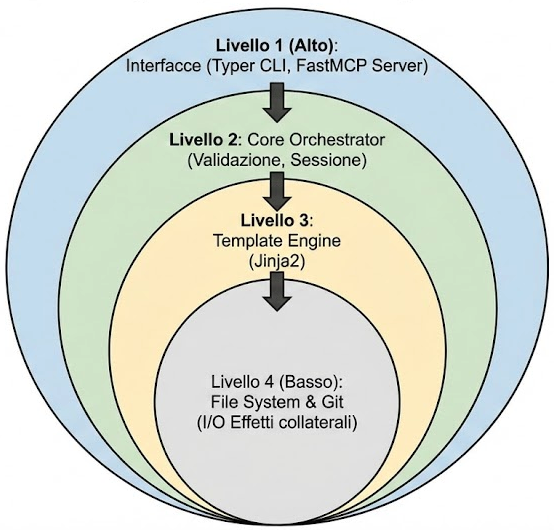
\includegraphics[width=0.6\textwidth]{images/strati_forge.png}
    \caption{Separazione delle responsabilità di service-forge [Elaborazione dell'autore].}
    \label{fig:onion_forge}
\end{figure}

A livello architetturale, il sistema concretizza la sua logica tramite pattern di progettazione consolidati. La Dependency Injection disaccoppia i componenti per agevolarne il testing unitario. Un pattern Factory istanzia dinamicamente i generatori appropriati in base al profilo di progetto selezionato (es. API sincrona, worker ETL). La separazione tra la generazione dei contenuti testuali e la loro persistenza su disco è mediata da un pattern Observer, mentre l'astrazione Strategy permette di mutare il comportamento di scaffolding in funzione del dominio applicativo.

\subsection{Sviluppo della Command Line Interface (CLI)}
L'interfaccia a riga di comando, sviluppata tramite la libreria Typer \cite{Typer}, guida l'operatore nella composizione interattiva della configurazione di progetto. Il flusso di esecuzione procede sequenzialmente: parte dalla selezione del profilo architetturale e dalla definizione del percorso fisico, per poi richiedere la configurazione dei servizi AWS necessari e dei parametri del runtime serverless. A valle dell'inserimento, il sistema esegue una validazione formale prima di delegare al motore centrale la generazione degli artefatti.

La CLI funge esclusivamente da livello di presentazione. Non contenendo logiche di scaffolding codificate rigidamente, essa raccoglie l'input e lo trasferisce al livello sottostante. Questa delega totale assicura una rigorosa coerenza comportamentale tra l'esecuzione manuale da terminale e l'esecuzione automatizzata tramite assistenti IA.

\subsection{Esposizione dei tool tramite Model Context Protocol (MCP)}
L'integrazione del framework con gli assistenti basati su Large Language Models operanti negli IDE avviene tramite un server conforme al Model Context Protocol, implementato avvalendosi della libreria FastMCP. Il server espone due categorie di astrazioni: risorse in sola lettura per la scoperta dei profili architetturali supportati, e strumenti operativi (Tools) necessari per la configurazione e la generazione del codice sorgente.

Durante la fase di inizializzazione, il server inietta nell'agente conversazionale un set di istruzioni testuali di sistema. Come illustrato nel Listato \ref{lst:mcp-init}, queste direttive vincolano il modello logico a richiedere esplicitamente all'operatore umano i parametri infrastrutturali reali (es. identificativi dei bucket S3 o nomi delle tabelle DynamoDB), prevenendo categoricamente la generazione di codice cloud contenente valori placeholder.

\begin{lstlisting}[language=Python, caption={Inizializzazione del server FastMCP con iniezione delle direttive operative e dei vincoli per l'agente LLM}, label={lst:mcp-init}]
from fastmcp import FastMCP

mcp = FastMCP(
    "service-forge",
    instructions=(
        "Service Forge generates AWS Lambda-based microservices. "
        "Use get_profiles to discover available profiles and services. "
        "IMPORTANT: Every AWS service has configurable parameters. "
        "Never use default placeholder values without asking the user first. "
        "Use create_session to start, then configure_service. "
        "Be sure to run check_prerequisites first."
    ),
)
\end{lstlisting}

\subsection{Interazione deterministica con i Large Language Models}
Il disaccoppiamento introdotto dall'MCP presenta una sfida architetturale: la comunicazione tra l'LLM e il server locale è intrinsecamente stateless. Per forzare un'interazione deterministica e limitare le allucinazioni del modello, il sistema delega il controllo del flusso al server locale tramite quattro vincoli architetturali: l'imposizione di una sequenza operativa rigorosa, la validazione strutturata dei payload di configurazione tramite Pydantic, l'obbligo di formattare le risposte in formato JSON standardizzato e l'integrazione di una funzionalità di simulazione (dry-run) per ispezionare l'astrazione generata senza alterare il file system.

Per supportare la sequenzialità delle operazioni, il server implementa un registro in memoria che associa a ogni sessione di interazione un identificativo alfanumerico univoco. Il Listato \ref{lst:mcp-session-state} dimostra come l'invocazione dello strumento \texttt{create\_session} istanzi una struttura dati predefinita contenente le dipendenze AWS e le configurazioni del runtime.

\begin{lstlisting}[language=Python, caption={Gestione del ciclo di vita e dello stato di sessione in memoria all'interno del server MCP}, label={lst:mcp-session-state}]
import uuid
from typing import Dict, Any

_sessions: Dict[str, Dict[str, Any]] = {}

@mcp.tool()
def create_session() -> str:
    session_id = str(uuid.uuid4())[:8]
    _sessions[session_id] = {
        "aws_services": {},
        "included_services": [],
        "runtime": dict(GenerationEngine.DEFAULT_RUNTIME),
    }
    return _json({"session_id": session_id})
\end{lstlisting}

Ogni successiva invocazione di uno strumento di configurazione o generazione richiede il passaggio obbligatorio di tale \texttt{session\_id} e modifica esclusivamente la porzione di stato isolata. Questo paradigma operativo riduce le ambiguità contestuali e assicura che il processo di generazione del microservizio rimanga prevedibile e tracciabile, indipendentemente dall'ambiente di sviluppo integrato (IDE) adottato dallo sviluppatore.